\documentclass[tikz, border=10pt]{standalone}

\usepackage{tikz}
\usepackage{xcolor}

\begin{document}

% triangle spiral
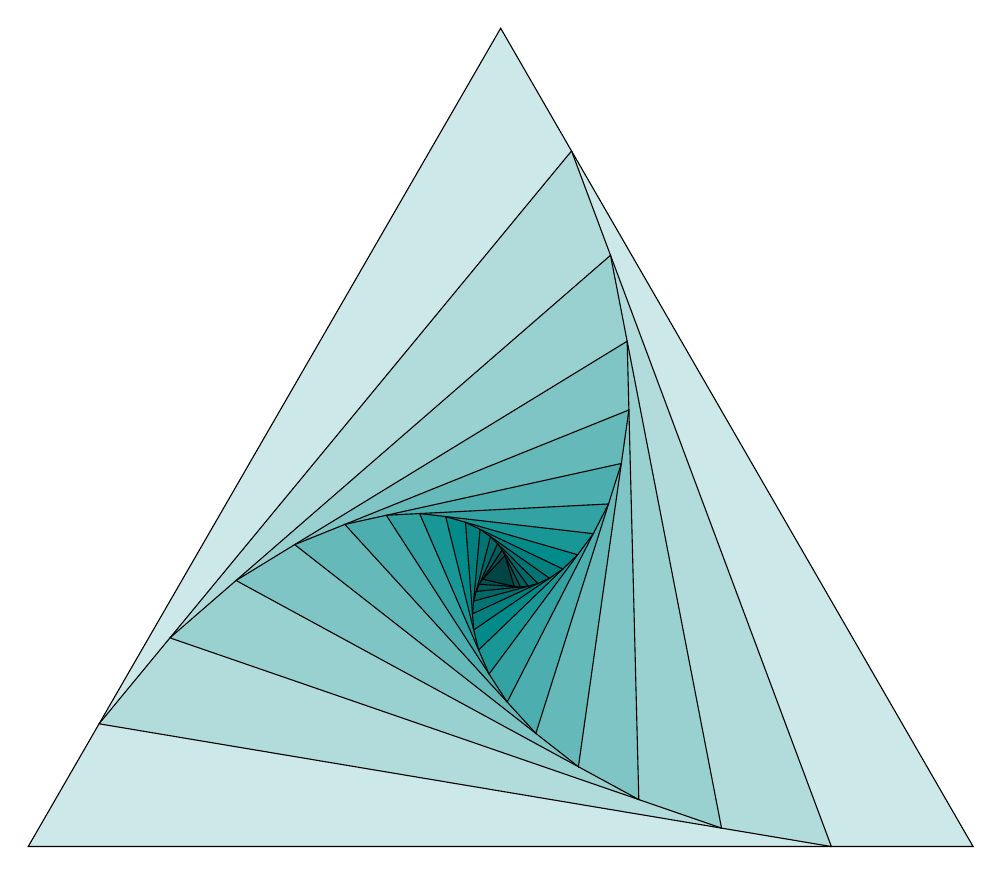
\begin{tikzpicture}
    \definecolor{DarkCyan}{HTML}{008b8b}
    \coordinate (A) at (0,0);
    \coordinate (B) at (-60:12cm);
    \coordinate (C) at (240:12cm);
    \foreach \density in {20,30,...,160}{%
        \draw[fill=DarkCyan!\density] (A)--(B)--(C)--cycle;
        \path
             (A) coordinate (X)
          -- (B) coordinate[pos=.15](A)
          -- (C) coordinate[pos=.15](B)
          -- (X) coordinate[pos=.15](C);
}
\end{tikzpicture}

% square spiral
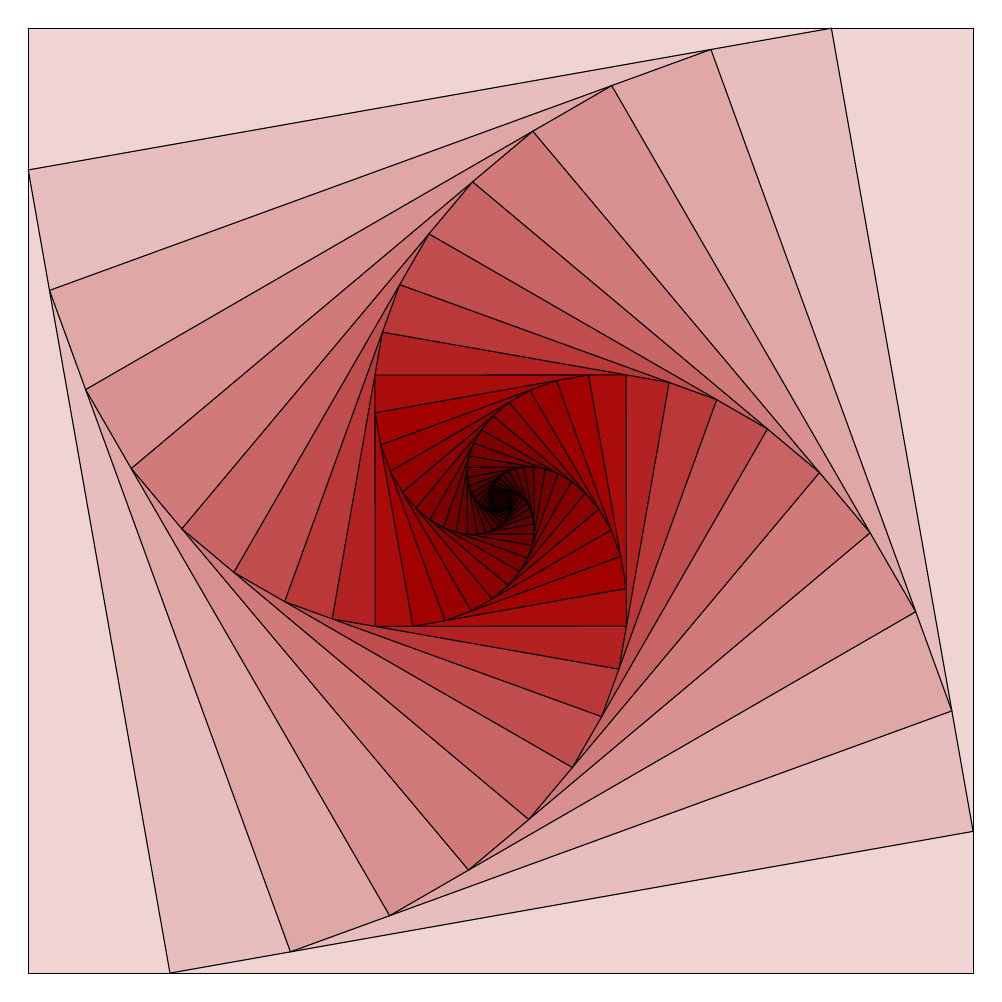
\begin{tikzpicture}
    \definecolor{FireBrick}{HTML}{b22222}
    \coordinate (A) at (0cm, 0cm);
    \coordinate (B) at (12cm, 0cm);
    \coordinate (C) at (12cm, 12cm);
    \coordinate (D) at (0cm, 12cm);
    \foreach \density in {20, 30, ..., 300}{
        \draw[fill=FireBrick!\density] (A) -- (B) -- (C) -- (D) -- cycle;
        \path (A) coordinate (X)
           -- (B) coordinate[pos=0.15] (A)
           -- (C) coordinate[pos=0.15] (B)
           -- (D) coordinate[pos=0.15] (C)
           -- (X) coordinate[pos=0.15] (D);
    }
\end{tikzpicture}

% polygon spiral (5 sides)
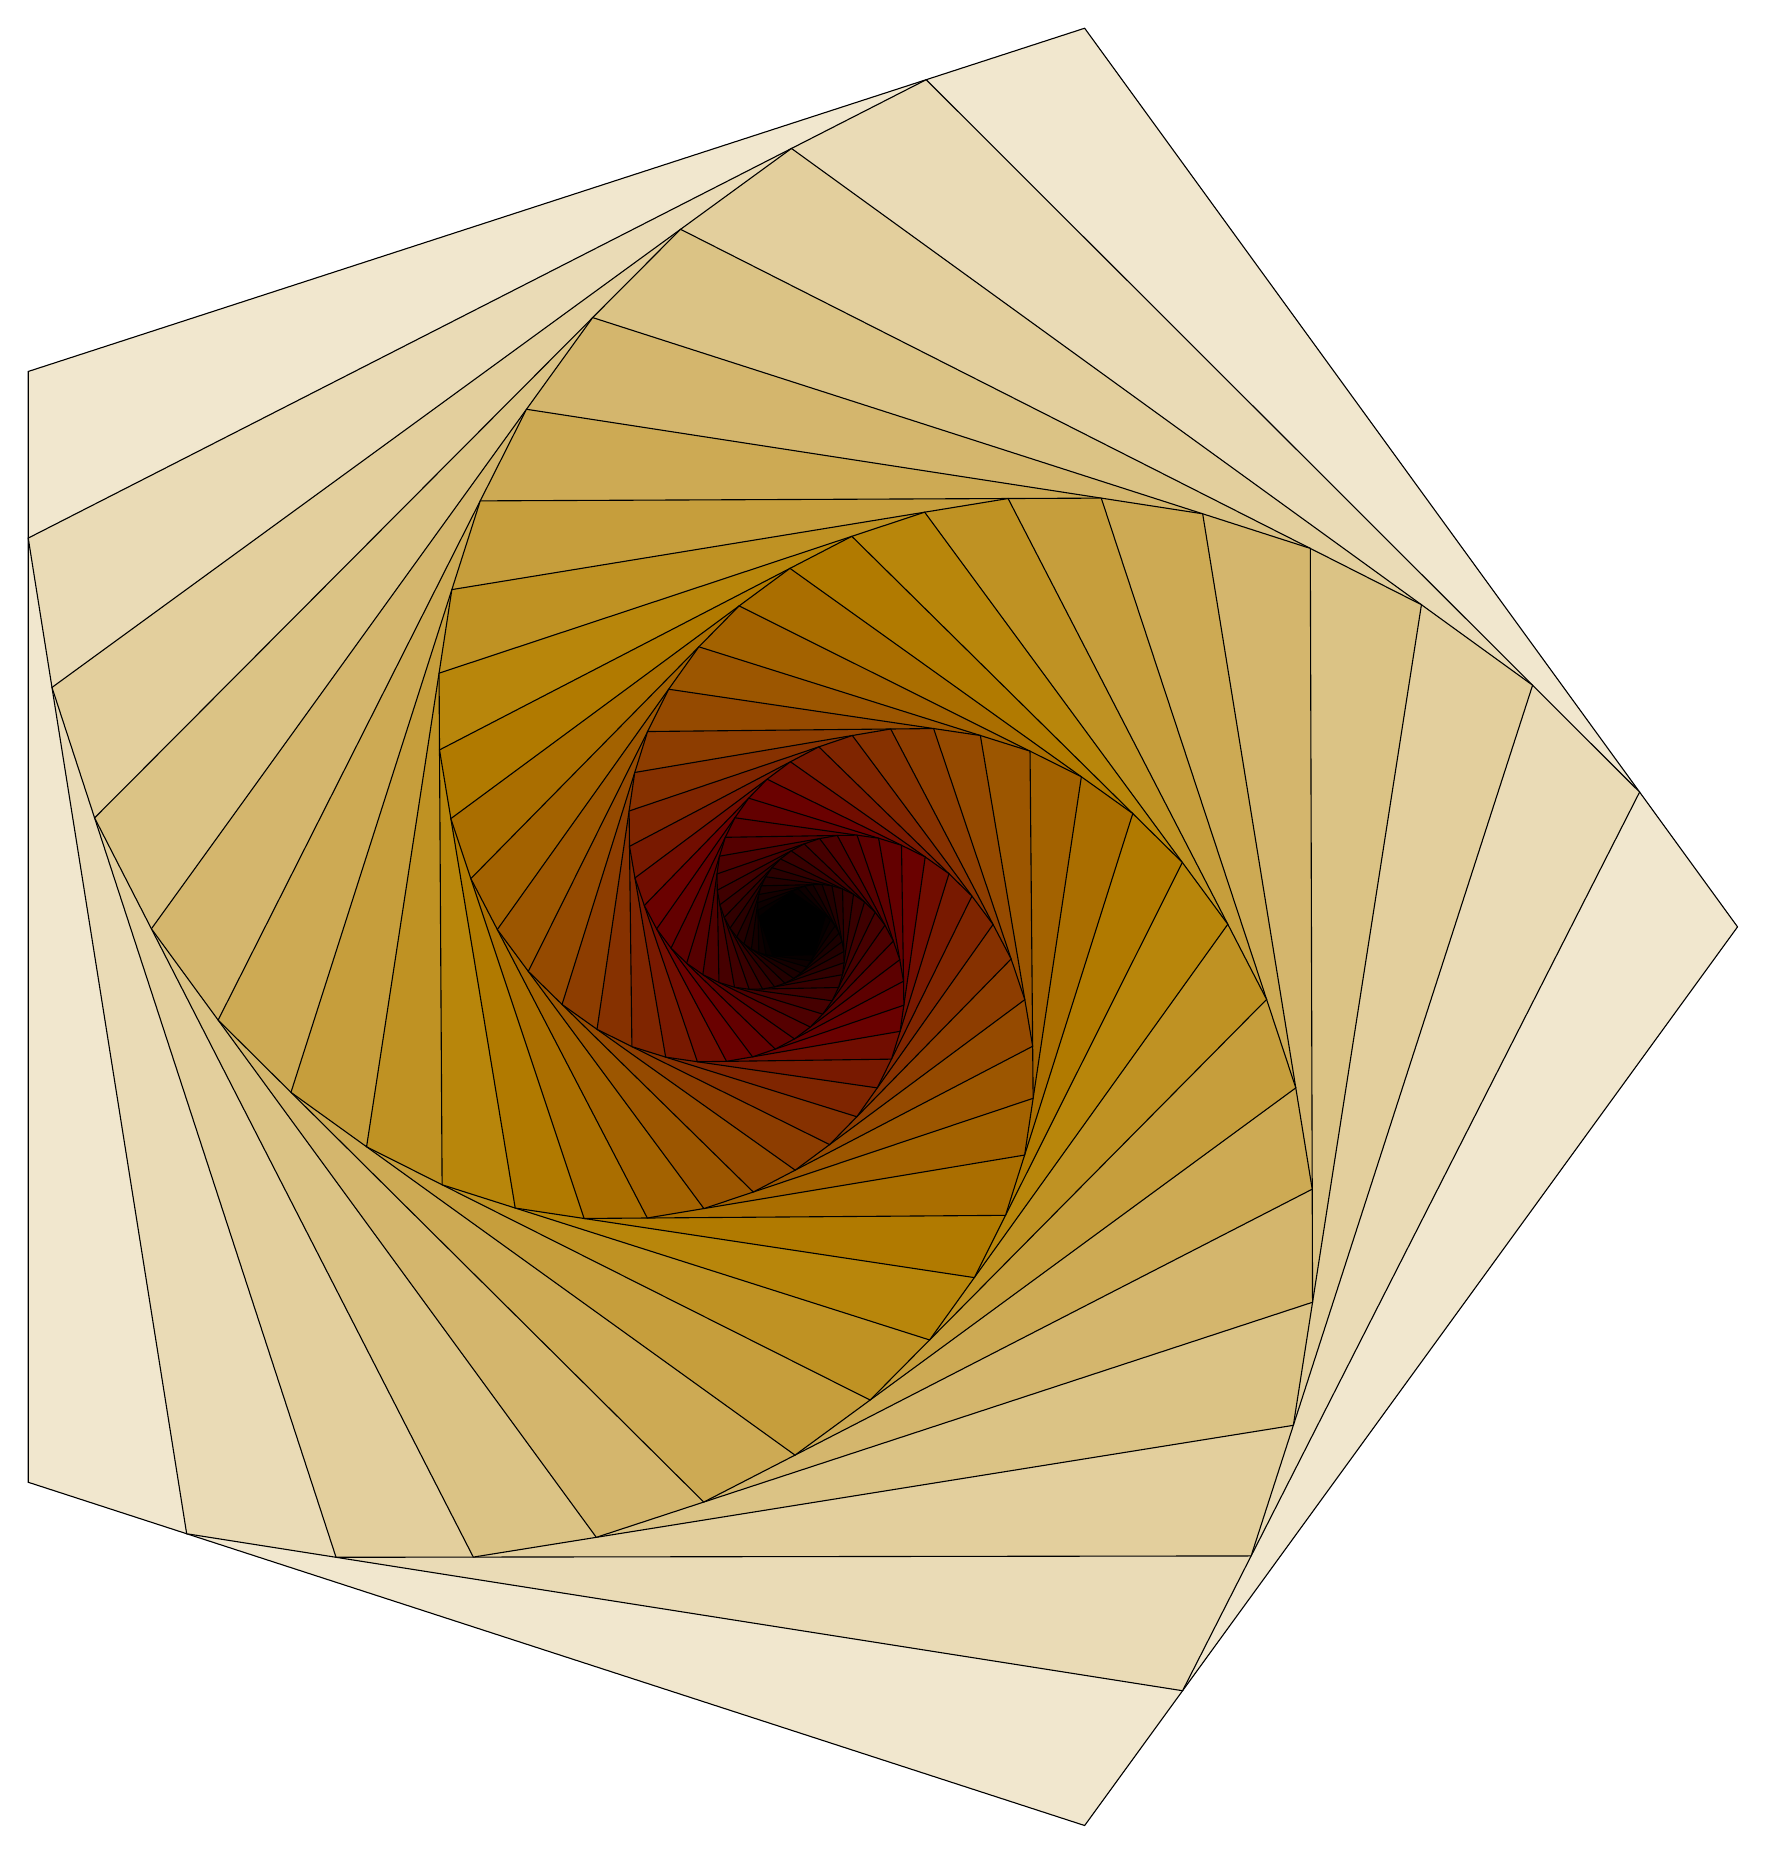
\begin{tikzpicture}
    \definecolor{DarkGoldenrod}{HTML}{b8860b}
    \coordinate (A) at (0:12cm);
    \coordinate (B) at (72:12cm);
    \coordinate (C) at (144:12cm);
    \coordinate (D) at (216:12cm);
    \coordinate (E) at (288:12cm);
    \foreach \density in {20, 30, ..., 400}{
        \draw[fill=DarkGoldenrod!\density] (A) -- (B) -- (C) -- (D) -- (E) -- cycle;
            \path (A) coordinate (X)
               -- (B) coordinate[pos=0.15] (A)
               -- (C) coordinate[pos=0.15] (B)
               -- (D) coordinate[pos=0.15] (C)
               -- (E) coordinate[pos=0.15] (D)
               -- (X) coordinate[pos=0.15] (E);
    }
\end{tikzpicture}

% hexagon spiral
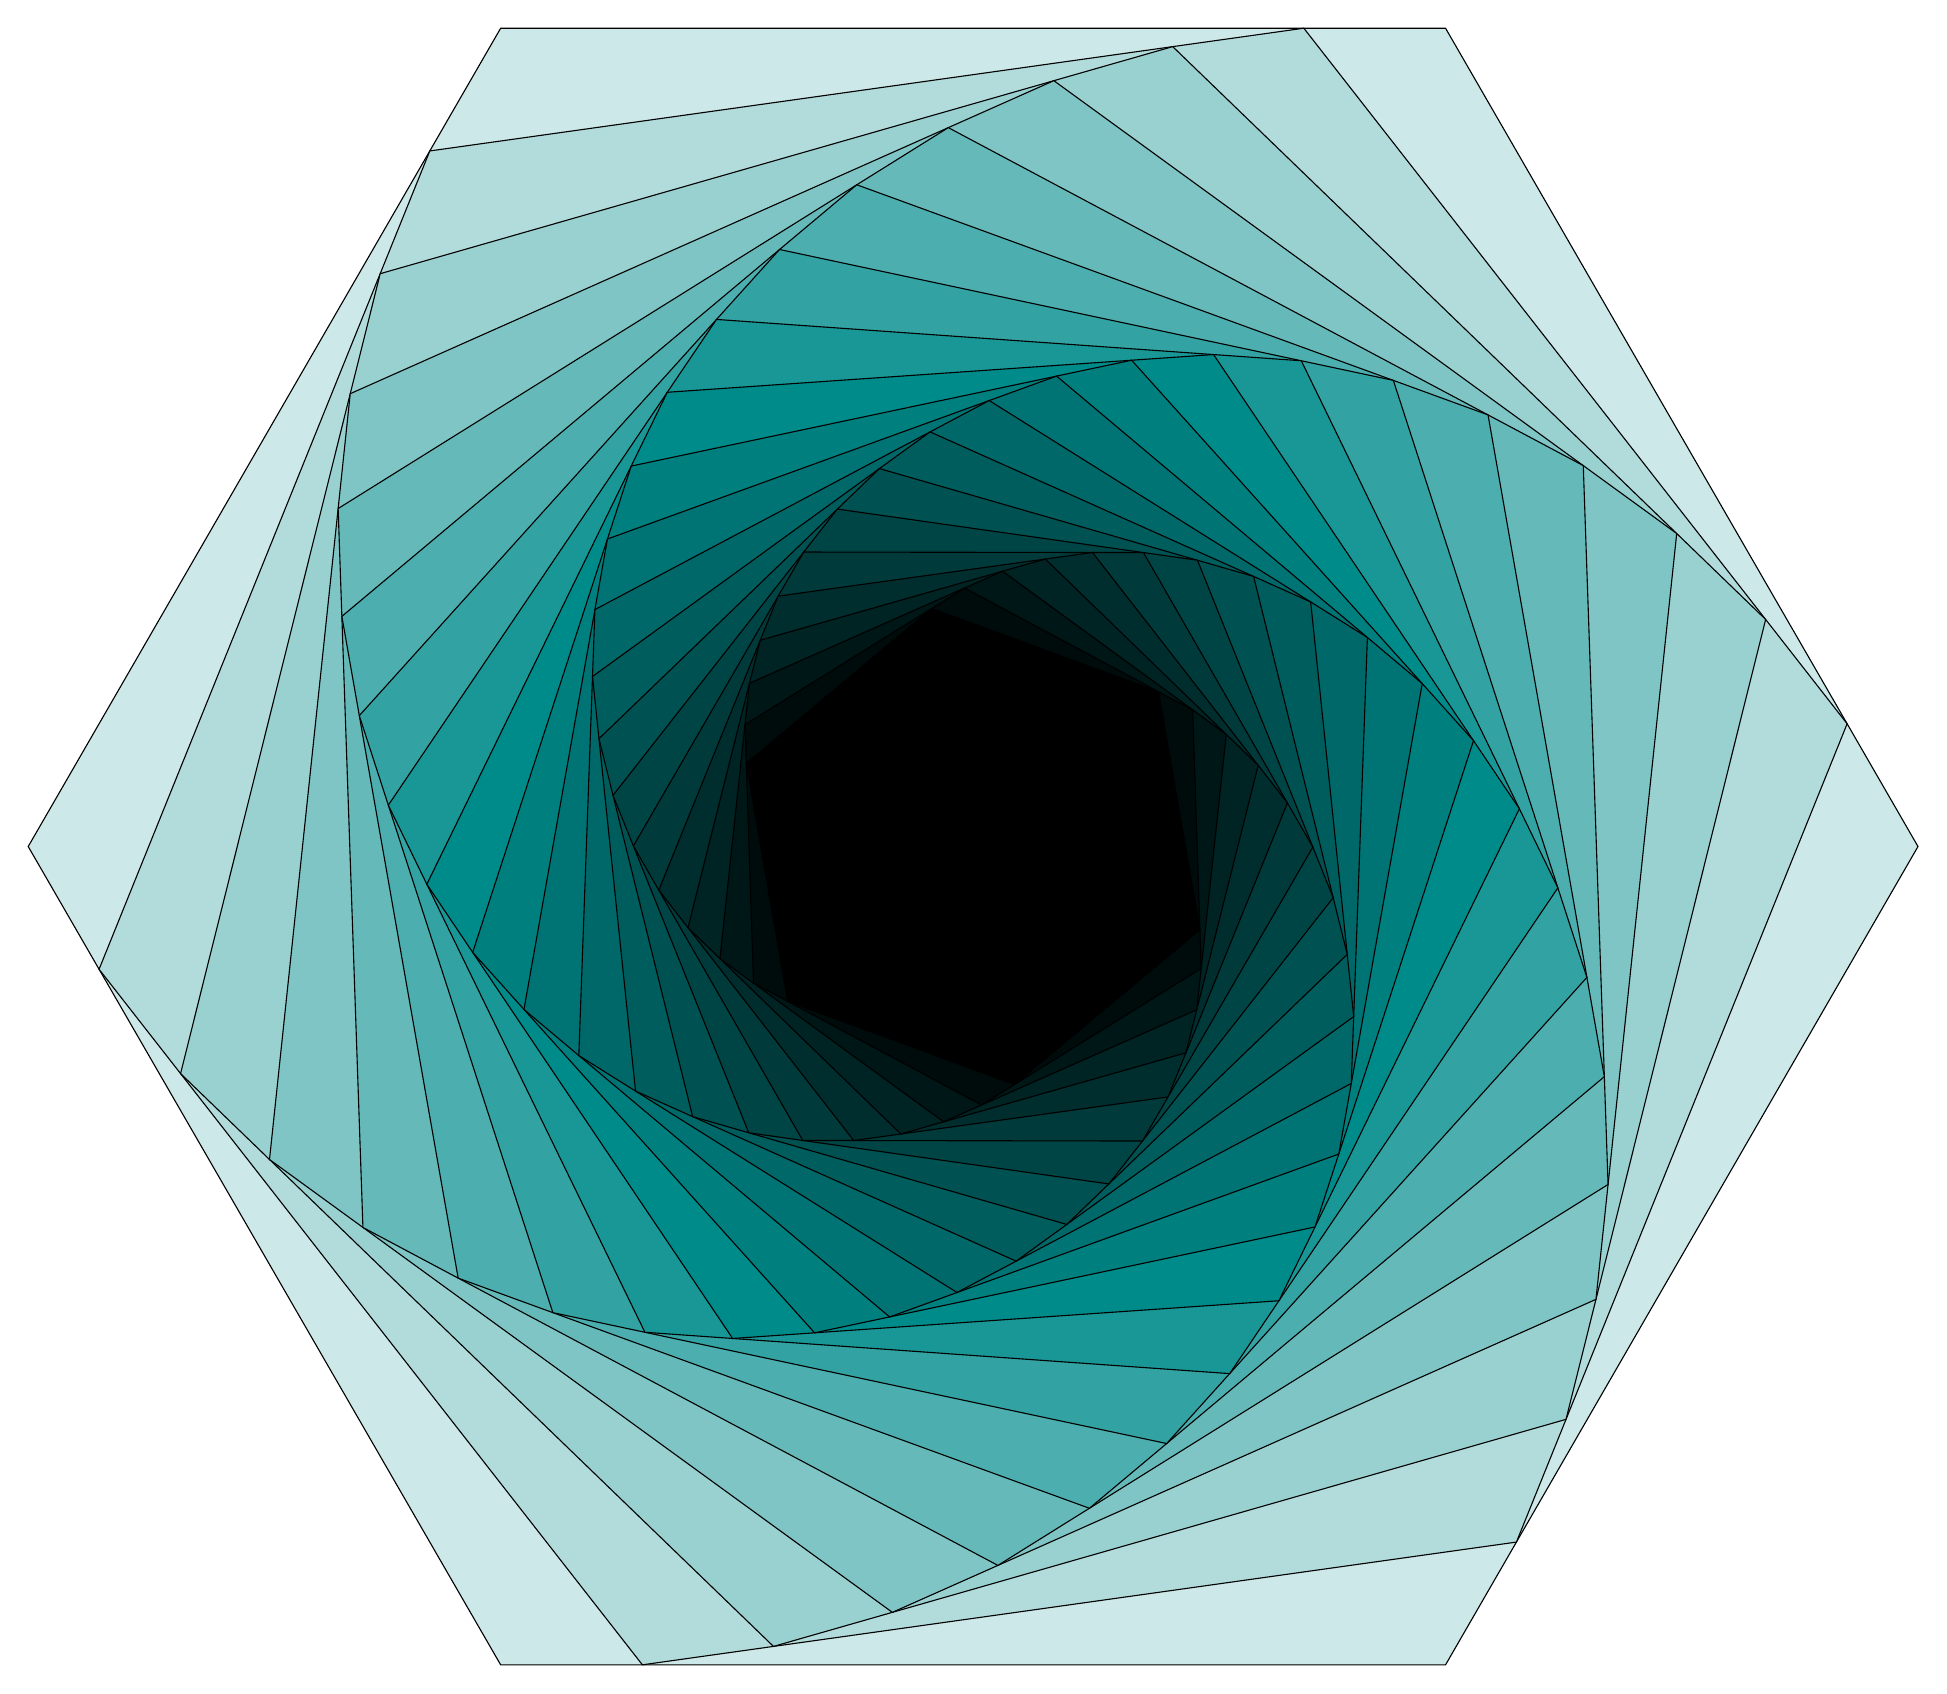
\begin{tikzpicture}
    \definecolor{DarkCyan}{HTML}{008b8b}
    \coordinate (A) at (0:12cm);
    \coordinate (B) at (60:12cm);
    \coordinate (C) at (120:12cm);
    \coordinate (D) at (180:12cm);
    \coordinate (E) at (240:12cm);
    \coordinate (F) at (300:12cm);
    \foreach \density in {20, 30, ..., 400}{
        \draw[fill=DarkCyan!\density] (A) -- (B) -- (C) -- (D) -- (E) -- (F) -- cycle;
            \path (A) coordinate (X)
               -- (B) coordinate[pos=0.15] (A)
               -- (C) coordinate[pos=0.15] (B)
               -- (D) coordinate[pos=0.15] (C)
               -- (E) coordinate[pos=0.15] (D)
               -- (F) coordinate[pos=0.15] (E)
               -- (X) coordinate[pos=0.15] (F);
    }
\end{tikzpicture}
\end{document}